\documentclass[aspectratio=169]{beamer}
\mode<presentation>

\usepackage{adjustbox}
\usepackage{amsmath}
\usepackage{array}
\usepackage{calc}
\usepackage{cancel}
\usepackage{etoolbox}
\usepackage{fancyvrb}
\usepackage{listings}
\usepackage[framemethod=tikz]{mdframed}
\usepackage{relsize}
\usepackage{graphicx}
\usepackage{stmaryrd}
\usepackage[most]{tcolorbox}
\usepackage[overlay,absolute]{textpos}
\usepackage{xcolor}

\usepackage{tikz}
\usetikzlibrary{arrows.meta}
\usetikzlibrary{calc}
\usetikzlibrary{positioning}
\usetikzlibrary{tikzmark}

\graphicspath{{../images}}

\usepackage{fontspec}
\setsansfont{Helvetica Neue Light}[
    BoldFont={Helvetica Neue Bold},
    BoldItalicFont={Helvetica Neue Bold Italic},
    ItalicFont={Helvetica Neue Light Italic}
]
\setmonofont{Iosevka Term}
\newfontface\helvreg{Helvetica Neue}

\renewcommand{\arraystretch}{1.2}
\renewcommand\UrlFont{\smaller[1]\tt}

\definecolor{grayish}{gray}{0.8}

\title{Concatenative programming and stack-based languages}
\author{Douglas Creager}
\institute{Walland Heavy Research}

\setbeamercolor{title}{fg=black}
\setbeamerfont{title}{series=\bfseries,size=\larger[1]}
\setbeamerfont{subtitle}{series=\mdseries,size=\smaller[2]}
\setbeamerfont{author}{size=\smaller[1]}
\setbeamerfont{institute}{size=\smaller[2]}
\setbeamertemplate{navigation symbols}{}
\setbeamercolor{frametitle}{fg=black}
\setbeamerfont{frametitle}{series=\bfseries}

% Picture credits

\makeatletter
\def\picturecredits{}
\newcommand{\picturecredit}[4]{
    \protected@xappto\picturecredits{
        \textsmaller[4]{Slide \theframenumber} &
        \textsmaller[3]{#1, “#2”} \vspace*{-0.6em} \newline
        \ifstrempty{#4}{\textsmaller[4]{#3}}{\textsmaller[4]{#3, \url{#4}}} \\[-0.4em]
    }
}
\makeatother

\newlength{\titlewidth}
\newcommand{\customtitle}[3]{
    \settowidth{\titlewidth}{#3}
    \begin{textblock*}{\titlewidth}(#1,#2)
        #3
    \end{textblock*}
}
\newcommand{\flattitle}[3]{\customtitle{#1}{#2}{\textbf{\LARGE #3}}}

\newcommand{\customshadowedtitle}[4]{
    \settowidth{\titlewidth}{#4}
    \addtolength{\titlewidth}{#3}
    \addtolength{\titlewidth}{0.1mm}
    \begin{textblock*}{\titlewidth}(#3+#1,#3+#2)
        #4
    \end{textblock*}
    \begin{textblock*}{\titlewidth}(#1,#2)
        \textcolor{white}{#4}
    \end{textblock*}
}
\newcommand{\shadowedtitle}[3]{\customshadowedtitle{#1}{#2}{0.4mm}{\textbf{\LARGE #3}}}

%%%%%%%%%%%%%%%%%%%%%%%%%%%%%%%%%%%%%%%%%%%%%%%%%%%%%%%%%%%%%%%%%%%%%%%%%%%%%%%%
% True centering of beamer slides

\makeatletter
\define@key{beamerframe}{c}[true]{% centered
  \beamer@frametopskip=0pt plus 1fill\relax%
  \beamer@framebottomskip=0pt plus 1fill\relax%
  \beamer@frametopskipautobreak=0pt plus .4\paperheight\relax%
  \beamer@framebottomskipautobreak=0pt plus .6\paperheight\relax%
  \def\beamer@initfirstlineunskip{}%
}
\makeatother

%%%%%%%%%%%%%%%%%%%%%%%%%%%%%%%%%%%%%%%%%%%%%%%%%%%%%%%%%%%%%%%%%%%%%%%%%%%%%%%%
% Explicit control of overlay-style visibility

% cf https://tex.stackexchange.com/a/512131

\makeatletter
\newcommand\pgfinvisible{\pgfsys@begininvisible}
\newcommand\pgfshown{\pgfsys@endinvisible}
\makeatother

%%%%%%%%%%%%%%%%%%%%%%%%%%%%%%%%%%%%%%%%%%%%%%%%%%%%%%%%%%%%%%%%%%%%%%%%%%%%%%%%
% Program source

\lstset{
  basicstyle=\small\ttfamily,%
  columns=fullflexible,
  keepspaces=true,
  escapechar=?,
  extendedchars=true}

\newcommand{\highlightsrc}[1]{%
    \tikz[remember picture]{
      \draw [overlay, draw=none, fill=blue!25]
        ([xshift=-1pt, yshift=8pt] pic cs:#1_start)
        rectangle
        ([xshift=1pt, yshift=-2pt] pic cs:#1_end)
        ;
    }%
    \ignorespaces
}

%%%%%%%%%%%%%%%%%%%%%%%%%%%%%%%%%%%%%%%%%%%%%%%%%%%%%%%%%%%%%%%%%%%%%%%%%%%%%%%%
% Environment frames

% Note that to use beamer overlays to ADD NEW rows to a tikz matrix, you need to
% put the TRAILING ROW'S closing \\ inside the \only, instead of the NEW ROW'S.
% c.f. https://tex.stackexchange.com/a/153797

\tikzset{
    envframe/.style={
        ampersand replacement=\&,
        draw=black,
        thick,
        rounded corners,
        fill=white,
        inner ysep=0.1em,
        row sep=-0.1em,
        every outer matrix/.append style={inner xsep=0.2em,inner ysep=0.2em},
        column 1/.style={
            sharp corners,
            anchor=base west,
        },
        column 2/.style={
            anchor=base,
            font=\small,
        },
    },
}

\tikzset{
    frame name/.style={
        execute at end node=\strut,
        font=\ttfamily\footnotesize\bfseries,
    },
    frame special/.style={
        execute at end node=\strut,
        font=\itshape\scriptsize,
    },
}

\tikzset{
    highlight node/.style={fill=red!25},
    highlight node on/.code args={<#1>}{%
        \alt<#1>{\pgfkeysalso{highlight node}}{}%
    }
}

%%%%%%%%%%%%%%%%%%%%%%%%%%%%%%%%%%%%%%%%%%%%%%%%%%%%%%%%%%%%%%%%%%%%%%%%%%%%%%%%
% Simple stack language

\newdimen\origiwspc
\origiwspc=\fontdimen2\font

\newcommand<>{\stackex}[2]{%
    \begin{onlyenv}#3
    \begin{tabular}[c]{
        @{\extracolsep{1em}}
        >{\rule[-0.6\baselineskip]{0pt}{1.8\baselineskip}\raggedleft\arraybackslash\fontdimen2\font=1ex}p{0.4\textwidth}<{\fontdimen2\font=\origiwspc}
        |
        >{\strut\raggedright\arraybackslash\leavevmode\color{blue}\ttfamily}p{0.5\textwidth}
    }
        \cline{1-1}
        \clipbox*{{\width - 0.4\textwidth} {-\depth} {\width} {\totalheight}}{#1} &
        \clipbox*{0pt {-\depth} {0.5\textwidth} {\totalheight}}{#2} \\
        \cline{1-1}
    \end{tabular}
    \end{onlyenv}%
    \ignorespaces
}

\newcommand{\val}[1]{\textcolor{black}{\textup{#1}}}
\newcommand{\sym}[1]{\textcolor{blue}{\texttt{#1}}}
\newcommand{\quot}[1]{\textcolor{blue}{\texttt{[#1]}}}
\newcommand{\mquot}[1]{\quot{\textcolor{black}{$#1$}}}
\newcommand{\eff}[1]{\textcolor{gray}{\texttt{\textit{#1}}}}

\newcommand{\ssym}[1]{\sym{\textsmaller[1]{#1}}}
\newcommand{\combwhy}[1]{\textcolor{teal}{\textsf{\textbf{#1}}}}

\newcommand{\stacksplit}[2][]{%
    \tcbox[
        standard jigsaw,
        nobeforeafter,
        size=fbox,
        boxrule=0pt,
        sharp corners=all,
        colback=white!0,
        #1
    ]{\sym{\strut#2}}%
    \ignorespaces
}

\newcommand{\compilestack}[1]{
    \lcompile \text{\raisebox{-0.75em}{\ignorespaces #1}} \rcompile
}

\newcommand<>{\stackeffect}[2]{%
    \begin{onlyenv}#3%
        \begin{center}
        \begin{tabular}{l}
            \eff{#1} \\
            \sym{#2} \\
        \end{tabular}%
        \end{center}%
    \end{onlyenv}%
    \ignorespaces
}

\newcommand<>{\interp}[2]{%
    \begin{onlyenv}#3%
        \begin{center}
        \begin{tabular}{ccp{60mm}}
            \sym{#1} & $\Longrightarrow$ &
            \textcolor{gray}{\textit{\ignorespaces #2}} \\
        \end{tabular}%
        \end{center}%
    \end{onlyenv}%
    \ignorespaces
}

\newcommand{\highlightmath}[2][blue!25]{%
    \tikz[remember picture]{
      \draw [overlay, draw=none, fill=#1]
        ([xshift=-1pt, yshift=12pt] pic cs:#2_start)
        rectangle
        ([xshift=1pt, yshift=-6pt] pic cs:#2_end)
        ;
    }%
    \ignorespaces
}

\newcommand\defalt{\mathrel{\:\mid\:}}
\newcommand\defeq{\mathrel{\,\triangleq\,}}
\newcommand\qeq{\mathrel{\stackrel{\mathrm{?}}{=}}}
\newcommand\veq{\mathrel{\rotatebox{90}{$=$}}}
\newcommand\yeq{\mathrel{\stackrel{\checkmark}{=}}}
\newcommand\withsub[1]{{\scriptscriptstyle #1}}

\newcommand{\eval}[1]{\ensuremath{\llbracket \sym{#1} \rrbracket}}
\newcommand\builtin{\textcolor{black}{\textsf{\textit{builtin}}}}
\newcommand\lit{\textcolor{black}{\textsf{\textit{literal}}}}
\newcommand\insn{\textcolor{black}{\textsf{\textit{instruction}}}}
\newcommand\prog{\textcolor{black}{\textsf{\textit{program}}}}

\newcommand\qqq{\raisebox{-0.2em}{\textsf{\textbf{\larger[2] ?}}}}

%%%%%%%%%%%%%%%%%%%%%%%%%%%%%%%%%%%%%%%%%%%%%%%%%%%%%%%%%%%%%%%%%%%%%%%%%%%%%%%%
% Compiling

\newcommand\lcompile{\mathopen{{\langle}\mkern-3.5mu{|}}}
\newcommand\rcompile{\mathclose{{|}\mkern-3.5mu{\rangle}}}
\newcommand\concat{\mathbin{+\mkern-10mu+}}

\newcommand\compiled[2][lightgray]{%
    \adjustbox{bgcolor=#1,minipage=20mm,margin=2pt}{\ttfamily\smaller[3]\begin{tabular}{@{~}l@{~}}#2\end{tabular}}%
    \ignorespaces
}

%%%%%%%%%%%%%%%%%%%%%%%%%%%%%%%%%%%%%%%%%%%%%%%%%%%%%%%%%%%%%%%%%%%%%%%%%%%%%%%%
% Lambda calculus

\newcommand\ldot{\mathop{\text{.}}}

%%%%%%%%%%%%%%%%%%%%%%%%%%%%%%%%%%%%%%%%%%%%%%%%%%%%%%%%%%%%%%%%%%%%%%%%%%%%%%%%
% SKI calculus

\newcommand\Sc{\textsf{\textbf{S}}}
\newcommand\Kc{\textsf{\textbf{K}}}
\newcommand\Ic{\textsf{\textbf{I}}}

%%%%%%%%%%%%%%%%%%%%%%%%%%%%%%%%%%%%%%%%%%%%%%%%%%%%%%%%%%%%%%%%%%%%%%%%%%%%%%%%
% Math equation spacing

\newcommand{\zerodisplayskips}{%
  \abovedisplayskip=0pt
  \belowdisplayskip=0pt
  \abovedisplayshortskip=0pt
  \belowdisplayshortskip=0pt
}
\newcommand{\removedisplayskips}{%
  \appto\normalsize{\zerodisplayskips}
  \appto\small{\zerodisplayskips}
  \zerodisplayskips
}

%%%%%%%%%%%%%%%%%%%%%%%%%%%%%%%%%%%%%%%%%%%%%%%%%%%%%%%%%%%%%%%%%%%%%%%%%%%%%%%%
% Citations

\newcommand<>{\citepaper}[1]{%
    \begin{textblock*}{0pt}(0pt,0pt)
    \begin{onlyenv}#2%
    \begin{tikzpicture}[remember picture,overlay]
        \node[
            anchor=south, yshift=1em,
            draw, thick,
            inner sep=0.6em,
            text width=90mm,
            align=flush left,
            node font={\rmfamily\smaller[2]},
        ] at (current page.south) {#1};
    \end{tikzpicture}%
    \end{onlyenv}%
    \end{textblock*}%
    \ignorespaces
}

%%%%%%%%%%%%%%%%%%%%%%%%%%%%%%%%%%%%%%%%%%%%%%%%%%%%%%%%%%%%%%%%%%%%%%%%%%%%%%%%

\begin{document}

\begin{frame}
    \begin{textblock*}{160mm}(0mm,0mm)
        \picturecredit{Douglas Creager}{Laurel Valley}{All rights reserved}{}
        \adjincludegraphics[Trim=13.5in 0.25in 15in 11in, width=160mm]{laurel-valley.jpg}
    \end{textblock*}
    \customshadowedtitle{80mm - 0.5\titlewidth}{61mm}{0.2mm}{\textbf{\textlarger[1]{\inserttitle}}}
    \customshadowedtitle{80mm - 0.5\titlewidth}{69mm}{0.2mm}{\textsmaller[1]{\insertauthor}}
    \customshadowedtitle{80mm - 0.5\titlewidth}{73mm}{0.2mm}{\textsmaller[2]{\insertinstitute}}
    \customshadowedtitle{80mm - 0.5\titlewidth}{79mm}{0.2mm}{\textsmaller[2]{Strange Loop – Papers We Love}}
    \customshadowedtitle{80mm - 0.5\titlewidth}{82.5mm}{0.2mm}{\textsmaller[3]{September 21–22, 2023 – St. Louis}}
\end{frame}

%%%%%%%%%%%%%%%%%%%%%%%%%%%%%%%%%%%%%%%%%%%%%%%%%%%%%%%%%%%%%%%%%%%%%%%%%%%%%%%%
% § Names

\section{Names}

\begin{frame}
    \begin{textblock*}{160mm}(0mm,0mm)
        \picturecredit{peagreengirl}{Very Old payroll Journal}{CC-BY-2.0}{https://flic.kr/p/B2YPU}
        \adjincludegraphics[Trim=0.25in, width=160mm]{old-ledger.jpg}
    \end{textblock*}
    \shadowedtitle{150mm - \titlewidth}{10mm}{Names}
\end{frame}

\subsection{Python expression}

\begin{frame}[fragile]
    \frametitle{Pythagoras}
    \begin{columns}[c]
        \begin{column}{90mm}%
        \centering%
        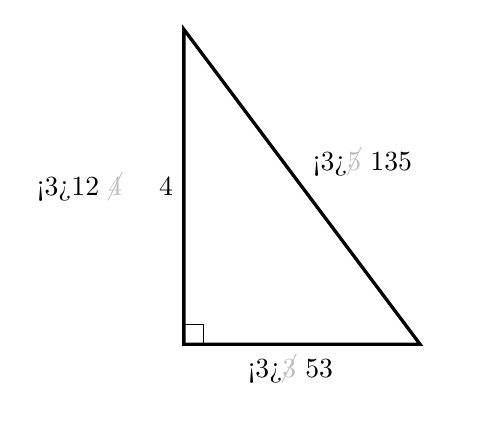
\begin{tikzpicture}[baseline={(current bounding box.center)}]
            \draw[very thick]
              (0,0) -- node[left] {\alt<3>{12~\textcolor{lightgray}{\cancel{4}}}{\phantom{12~}4}}
              (0,4) -- node[above right] {\alt<3>{\textcolor{lightgray}{\cancel{5}}~13}{5\phantom{~13}}}
              (3,0) -- node[below] {\alt<3>{\textcolor{lightgray}{\cancel{3}}~5}{3\vphantom{\cancel{3}}\phantom{~5}}} cycle;
            \draw[thin] (0,0.25) -- (0.25,0.25) -- (0.25,0);
        \end{tikzpicture}
        \end{column}%
        \begin{column}{70mm}%
        \begin{onlyenv}<1-2>%
        \begin{lstlisting}[language=python,gobble=8]
        import math

        leg1 = 3
        leg2 = 4

        l1sq = leg1 * leg1
        l2sq = leg2 * leg2
        hypotsq = l1sq + l2sq
        result = math.sqrt(hypotsq)

        print(result)
        \end{lstlisting}%
        \begin{uncoverenv}<2>%
        \begin{lstlisting}[gobble=8,basicstyle={\color{blue}\ttfamily\larger[1]}]
        5
        \end{lstlisting}%
        \end{uncoverenv}%
        \end{onlyenv}%
        \begin{onlyenv}<3>%
        \begin{lstlisting}[language=python,gobble=8]
        import math

        def pythogoras(leg1, leg2):
            l1sq = leg1 * leg1
            l2sq = leg2 * leg2
            hypotsq = l1sq + l2sq
            return math.sqrt(hypotsq)

        print(pythagoras(3, 4))
        print(pythagoras(5, 12))
        \end{lstlisting}%
        \pgfinvisible%
        \begin{lstlisting}[gobble=8,basicstyle={\color{blue}\ttfamily\larger[1]},belowskip=0pt]
        5
        \end{lstlisting}%
        \begin{lstlisting}[gobble=8,basicstyle={\color{blue}\ttfamily\larger[1]},aboveskip=0pt]
        13
        \end{lstlisting}%
        \pgfshown%
        \end{onlyenv}%
        \end{column}%
    \end{columns}%
\end{frame}

\subsection{Python function}

\begin{frame}[fragile]
    \frametitle{Pythagoras}
    \begin{columns}[c]
        \begin{column}{90mm}%
        \only<2-3>  {\highlightsrc{math}}%
        \only<4>    {\highlightsrc{pyth}}%
        \only<5>    {\highlightsrc{formals}}%
        \only<5-9>  {\highlightsrc{actuals1}}%
        \only<6>    {\highlightsrc{s1}}%
        \only<7>    {\highlightsrc{s2}}%
        \only<8>    {\highlightsrc{s3}}%
        \only<9>    {\highlightsrc{s4}}%
        \only<11-15>{\highlightsrc{actuals2}}%
        \only<12>   {\highlightsrc{s1}}%
        \only<13>   {\highlightsrc{s2}}%
        \only<14>   {\highlightsrc{s3}}%
        \only<15>   {\highlightsrc{s4}}%
        \centering%
        \begin{tikzpicture}[
            remember picture,
            every node/.style={node distance=0.5cm},
        ]
        \matrix[envframe] (mod) {
            \only<1>{\node[inner sep=0.6em]{};}
            \only<2- >{
                \node[frame name,highlight node on={<9>}]{math}; \&
                \node[frame special] (math) {math module};
            }
            \only<4- >{ \\
                \node[frame name,highlight node on={<5>}]{pythagoras}; \&
                \node[frame special]{pythagoras function};
            }
            \\
        };
        \only<3- >{
            \matrix[envframe,above=of mod] (mathframe) {
                \& \node{$\cdots$}; \\
                \node[frame name,highlight node on={<9>}]{sqrt}; \&
                \node[frame special]{sqrt function}; \\
                \& \node{$\cdots$}; \\
            };
        }
        \only<3>{
            \draw [overlay, thick, -{Triangle[]}]
              (math.east) .. controls +(0:1cm) and +(0:1cm) ..
              (mathframe.east);
        }
        \only<4- >{
            \draw [overlay, thick, -{Triangle[]}]
              (math.east) .. controls +(0:0.75cm) and +(0:1.25cm) ..
              (mathframe.east);
        }
        \only<5-9>{
            \matrix[envframe,below=of mod] (call1) {
                \only<5-9>{
                    \node[frame name, highlight node on={<6>}]{leg1}; \& \node{3}; \\
                    \node[frame name, highlight node on={<7>}]{leg2}; \& \node{4};
                }
                \only<6-9>{ \\
                    \node[frame name, highlight node on={<8>}]{l1sq}; \& \node{9};
                }
                \only<7-9>{ \\
                    \node[frame name, highlight node on={<8>}]{l2sq}; \& \node{16};
                }
                \only<8-9>{ \\
                    \node[frame name,highlight node on={<9>}]{hypotsq}; \& \node{25};
                }
                \\
            };
            \draw[densely dashed, thick, ->] (call1.north) -- (mod.south);
        }
        \only<11-15>{
            \matrix[envframe,below=of mod] (call1) {
                \only<11-16>{
                    \node[frame name, highlight node on={<12>}]{leg1}; \& \node{5}; \\
                    \node[frame name, highlight node on={<13>}]{leg2}; \& \node{12};
                }
                \only<12-16>{ \\
                    \node[frame name, highlight node on={<14>}]{l1sq}; \& \node{25};
                }
                \only<13-16>{ \\
                    \node[frame name, highlight node on={<14>}]{l2sq}; \& \node{144};
                }
                \only<14-16>{ \\
                    \node[frame name,highlight node on={<15>}]{hypotsq}; \& \node{169};
                }
                \\
            };
            \draw[densely dashed, thick, ->] (call1.north) -- (mod.south);
        }
        \end{tikzpicture}%
        \end{column}%
        \begin{column}{70mm}%
        \begin{lstlisting}[language=python,gobble=8]
        ?\tikzmark{math_start}?import math?\tikzmark{math_end}?

        ?\tikzmark{pyth_start}?def ?\tikzmark{formals_start}?pythogoras(leg1, leg2)?\tikzmark{formals_end}?:
            ?\tikzmark{s1_start}?l1sq = leg1 * leg1?\tikzmark{s1_end}?
            ?\tikzmark{s2_start}?l2sq = leg2 * leg2?\tikzmark{s2_end}?
            ?\tikzmark{s3_start}?hypotsq = l1sq + l2sq?\tikzmark{s3_end}?
            return ?\tikzmark{s4_start}?math.sqrt(hypotsq)?\tikzmark{pyth_end}\tikzmark{s4_end}?

        print(?\tikzmark{actuals1_start}?pythagoras(3, 4)?\tikzmark{actuals1_end}?)
        print(?\tikzmark{actuals2_start}?pythagoras(5, 12)?\tikzmark{actuals2_end}?)
        \end{lstlisting}%
        \begin{uncoverenv}<10->%
        \begin{lstlisting}[gobble=8,basicstyle={\color{blue}\ttfamily\larger[1]},belowskip=0pt]
        5
        \end{lstlisting}%
        \end{uncoverenv}%
        \begin{uncoverenv}<16->%
        \begin{lstlisting}[gobble=8,basicstyle={\color{blue}\ttfamily\larger[1]},aboveskip=0pt]
        13
        \end{lstlisting}%
        \end{uncoverenv}%
        \end{column}%
    \end{columns}%
\end{frame}

%%%%%%%%%%%%%%%%%%%%%%%%%%%%%%%%%%%%%%%%%%%%%%%%%%%%%%%%%%%%%%%%%%%%%%%%%%%%%%%%
% § Stack-based languages

\section{Stack-based languages}

\begin{frame}
    \begin{textblock*}{160mm}(0mm,0mm)
        \picturecredit{Marco Verch}{Stack of pancakes with berries on a plate}{CC-BY-2.0}{https://flic.kr/p/2jYUh8M}
        \includegraphics[width=180mm]{pancakes.jpg}
    \end{textblock*}
    \flattitle{150mm - \titlewidth}{5mm}{Stack-based languages}
\end{frame}

\subsection{Programs operate on a stack}

\begin{frame}
    \frametitle{Programs operate on a stack}
    \stackex<+>{       }{ }
    \stackex<+>{       }{ 1 2 + }
    \stackex<+>{      1}{ 2 + }
    \stackex<+>{    1 2}{ + }
    \stackex<+>{      3}{ }
\end{frame}

\subsection{Stack expression}

\begin{frame}
    \frametitle{Pythagoras}
    \stackex<+>{       }{ 3 3 * 4 4 * + sqrt }
    \stackex<+>{      3}{ 3 * 4 4 * + sqrt }
    \stackex<+>{    3 3}{ * 4 4 * + sqrt }
    \stackex<+>{      9}{ 4 4 * + sqrt }
    \stackex<+>{    9 4}{ 4 * + sqrt }
    \stackex<+>{  9 4 4}{ * + sqrt }
    \stackex<+>{   9 16}{ + sqrt }
    \stackex<+>{     25}{ sqrt }
    \stackex<+->{      5}{ }
    \begin{onlyenv}<+>
        \begin{tikzpicture}[remember picture,overlay]
            \node[anchor=center,draw,thick,inner sep=0mm]
                at ($(current page.center)!0.5!(current page.east)$) {
                \includegraphics[width=30mm]{hp-calculator.jpg}
            };
        \end{tikzpicture}
    \end{onlyenv}
\end{frame}
\picturecredit{striegel}{HP-48GX calculator}{CC-BY-2.0}{https://flic.kr/p/BWttzE}

\subsection{Manipulating the stack}

\begin{frame}
    \frametitle{Manipulating the stack}
    \stackex<+>{         }{ 3 4 dup * swap dup * + sqrt }
    \stackex<+>{        3}{ 4 dup * swap dup * + sqrt }
    \stackex<+>{      3 4}{ dup * swap dup * + sqrt }
    \stackex<+>{    3 4 4}{ * swap dup * + sqrt }
    \stackex<+>{     3 16}{ swap dup * + sqrt }
    \stackex<+>{     16 3}{ dup * + sqrt }
    \stackex<+>{   16 3 3}{ * + sqrt }
    \stackex<+>{     16 9}{ + sqrt }
    \stackex<+>{       25}{ sqrt }
    \stackex<+>{        5}{ }
\end{frame}

\subsection{Stack abstraction}

\begin{frame}
    \frametitle{Abstraction}
    \stackex<+>{         }{ 3 4 dup * swap dup * + sqrt }
    \stackex<+>{         }{ 3 4 \quot{dup * swap dup * + sqrt} apply }
    \stackex<+>{        3}{ 4 \quot{dup * swap dup * + sqrt} apply }
    \stackex<+>{      3 4}{ \quot{dup * swap dup * + sqrt} apply }
    \stackex<+>{      3 4 \quot{dup * swap dup * + sqrt}} { apply }
    \stackex<+>{      3 4}{ dup * swap dup * + sqrt }
    \stackex<+>{    3 4 4}{ * swap dup * + sqrt }
    \stackex<+>{     3 16}{ swap dup * + sqrt }
    \stackex<+>{     16 3}{ dup * + sqrt }
    \stackex<+>{   16 3 3}{ * + sqrt }
    \stackex<+>{     16 9}{ + sqrt }
    \stackex<+>{       25}{ sqrt }
    \stackex<+>{        5}{ }
\end{frame}

\subsection{Digging for dirt}

\begin{frame}
    \frametitle{Digging for dirt}
    \stackex<+>{         }{ \quot{dup * swap dup * + sqrt} 3 4 ??? apply }
    \stackex<+>{\quot{dup * swap dup * + sqrt}}{ 3 4 ??? apply }
    \stackex<+>{\quot{dup * swap dup * + sqrt} 3}{ 4 ??? apply }
    \stackex<+>{\quot{dup * swap dup * + sqrt} 3 4}{ ??? apply }
    \stackex<+>{\quot{dup * swap dup * + sqrt} 3 4}{ dig2 apply }
    \stackex<+>{3 4 \quot{dup * swap dup * + sqrt}}{ apply }
    \stackex<+>{      3 4}{ dup * swap dup * + sqrt }
    \stackex<+>{    3 4 4}{ * swap dup * + sqrt }
    \stackex<+>{     3 16}{ swap dup * + sqrt }
    \stackex<+>{     16 3}{ dup * + sqrt }
    \stackex<+>{   16 3 3}{ * + sqrt }
    \stackex<+>{     16 9}{ + sqrt }
    \stackex<+>{       25}{ sqrt }
    \stackex<+>{        5}{ }
\end{frame}

\subsection{Applying a quotation more than once}

\begin{frame}
    \frametitle{Applying a quotation more than once}

    \begin{onlyenv}<+-+(3)>
    \begin{center}
        \stacksplit[only=<+>{colback=gray!20}]{\quot{dup * swap dup * + sqrt}}
        \stacksplit[only=<+>{colback=gray!20}]{dup 3 4 dig2 apply drop}
        \stacksplit[only=<+>{colback=gray!20}]{5 12 dig2 apply drop}
    \end{center}
    \end{onlyenv}

    \stackex<+>{}{ \quot{dup * swap dup * + sqrt} dup 3 4 dig2 apply drop 5 12 dig2 apply drop }
    \stackex<+>{\quot{dup * swap dup * + sqrt}}{ dup 3 4 dig2 apply drop 5 12 dig2 apply drop }
    \stackex<+>{\quot{dup * swap dup * + sqrt} \quot{dup * swap dup * + sqrt}}{ 3 4 dig2 apply drop 5 12 dig2 apply drop }
    \stackex<+>{\quot{dup * swap dup * + sqrt} \quot{dup * swap dup * + sqrt} 3}{ 4 dig2 apply drop 5 12 dig2 apply drop }
    \stackex<+>{\quot{dup * swap dup * + sqrt} \quot{dup * swap dup * + sqrt} 3 4}{ dig2 apply drop 5 12 dig2 apply drop }
    \stackex<+>{\quot{dup * swap dup * + sqrt} 3 4 \quot{dup * swap dup * + sqrt}}{ apply drop 5 12 dig2 apply drop }
    \stackex<+>{\quot{dup * swap dup * + sqrt} 3 4}{ dup * swap dup * + sqrt drop 5 12 dig2 apply drop }
    \stackex<+>{\quot{dup * swap dup * + sqrt} 3 4 4}{ * swap dup * + sqrt drop 5 12 dig2 apply drop }
    \stackex<+>{\quot{dup * swap dup * + sqrt} 3 16}{ swap dup * + sqrt drop 5 12 dig2 apply drop }
    \stackex<+>{\quot{dup * swap dup * + sqrt} 16 3}{ dup * + sqrt drop 5 12 dig2 apply drop }
    \stackex<+>{\quot{dup * swap dup * + sqrt} 16 3 3}{ * + sqrt drop 5 12 dig2 apply drop }
    \stackex<+>{\quot{dup * swap dup * + sqrt} 16 9}{ + sqrt drop 5 12 dig2 apply drop }
    \stackex<+>{\quot{dup * swap dup * + sqrt} 25}{ sqrt drop 5 12 dig2 apply drop }
    \stackex<+>{\quot{dup * swap dup * + sqrt} 5}{ drop 5 12 dig2 apply drop }
    \stackex<+>{\quot{dup * swap dup * + sqrt}}{ 5 12 dig2 apply drop }
    \stackex<+>{\quot{dup * swap dup * + sqrt} 5}{ 12 dig2 apply drop }
    \stackex<+>{\quot{dup * swap dup * + sqrt} 5 12}{ dig2 apply drop }
    \stackex<+>{5 12 \quot{dup * swap dup * + sqrt}}{ apply drop }
    \stackex<+>{5 12}{ dup * swap dup * + sqrt drop }
    \stackex<+>{5 12 12}{ * swap dup * + sqrt drop }
    \stackex<+>{5 144}{ swap dup * + sqrt drop }
    \stackex<+>{144 5}{ dup * + sqrt drop }
    \stackex<+>{144 5 5}{ * + sqrt drop }
    \stackex<+>{144 25}{ + sqrt drop }
    \stackex<+>{169}{ sqrt drop }
    \stackex<+>{13}{ drop }
    \stackex<+>{}{ }
\end{frame}

%%%%%%%%%%%%%%%%%%%%%%%%%%%%%%%%%%%%%%%%%%%%%%%%%%%%%%%%%%%%%%%%%%%%%%%%%%%%%%%%
% § Meaning

\section{Meaning}

\begin{frame}
    \begin{textblock*}{160mm}(0mm,0mm)
        \picturecredit{Mustang Joe}{The Thinker}{Public domain}{https://flic.kr/p/a6gTRj}
        \adjincludegraphics[Trim=0.5in 0in, width=160mm]{thinker.jpg}
    \end{textblock*}
    \shadowedtitle{10mm}{10mm}{Meaning}
\end{frame}

\subsection{What is the meaning of a stack program?}

\begin{frame}
    \frametitle{What is the meaning of a stack program?}
    \stackex<+>{       }{ }
    \stackex<+>{       }{ 1 2 + }
    \stackex<+>{      1}{ 2 + }
    \stackex<+>{    1 2}{ + }
    \stackex<+>{      3}{ }
\end{frame}

\begin{frame}
    \frametitle{The stack doesn't have to start empty}
    \stackex<+>{    1337 42}{ 1 2 + }
    \stackex<+>{  1337 42 1}{ 2 + }
    \stackex<+>{1337 42 1 2}{ + }
    \stackex<+>{  1337 42 3}{ }
\end{frame}

\begin{frame}
    \interp<+>{1 2 +}{Push \val{3} onto the stack}
\end{frame}

\subsection{Programs can consume existing values}

\begin{frame}
    \frametitle{Programs can consume existing values}
    \stackex<+>{  1337 42 3}{ dup * }
    \stackex<+>{1337 42 3 3}{ * }
    \stackex<+>{  1337 42 9}{ }
\end{frame}

\begin{frame}
    \interp<+>{dup *}{
        Pop one value from the stack, square it, and push the result onto the
        stack
    }
\end{frame}

\subsection{Stack effects}

\begin{frame}[fragile]
    \frametitle{Stack effects}
    \citepaper{
        Slava Pestov, Daniel Ehrenberg, Joe Groff.
        “Factor: A Dynamic Stack-based Programming Language”.
        ACM SIGPLAN Notices 45:12. December 2010.
    }
    \stackeffect<+>{-- 3}{1 2 +}
    \stackeffect<+>{x -- x*x}{dup *}
    \stackeffect<+>{x -- result}{dup *}
\end{frame}

\subsection{Stack transformers}

\begin{frame}[t,fragile]
    \frametitle{More mathier}
    \removedisplayskips
    \begin{equation*}
    \begin{array}{c@{\quad}c@{\quad}l}
        \uncover<8->{i &\in& \mathbb{Z}} \\
        \uncover<8->{v &\defeq& i \defalt \quot{\prog}} \\
        \uncover<7->{\hat{v} &\defeq& \epsilon \defalt \hat{v} \cdot v} \\[2ex]
        \uncover<4->{\lit &\ni& \sym{0}, \sym{1}, \sym{42}, \ldots} \\
        \uncover<5->{
            \builtin &\defeq&
            \sym{+} \defalt \sym{*} \defalt \sym{sqrt} \defalt
            \sym{apply} \defalt \sym{dig2} \defalt \sym{drop} \defalt
            \sym{dup} \defalt \sym{swap} \defalt
            \ldots
        } \\
        \uncover<3->{
            \insn &\defeq&
            \lit \defalt
            \builtin \defalt
            \quot{\prog}
        } \\
        \uncover<2->{
            \prog &\defeq&
            \insn \defalt
            \prog~\prog
        } \\[2ex]
        \uncover<6->{
            \llbracket \prog \rrbracket &\in& \hat{v} \rightarrow \hat{v}
        } \\
    \end{array}%
    \end{equation*}%
    \citepaper{
        Manfred von Thun.
        “The mathematical foundations of Joy”.
        1994.
        \url{https://hypercubed.github.io/joy/html/j02maf.html}
    }
\end{frame}

\subsection{Evaluating stack programs}

\begin{frame}[t,fragile]
    \frametitle{Evaluating stack programs}
    \removedisplayskips
    \begin{columns}[t]
        \begin{column}<+->{60mm}
            \begin{uncoverenv}<+->
            \begin{equation*}
                \begin{array}{l@{\;\,}c@{\,\;}l}
                    \llbracket \sym{0} \rrbracket\ \hat{v} &=& \hat{v} \cdot \val{0} \\
                    \llbracket \sym{1} \rrbracket\ \hat{v} &=& \hat{v} \cdot \val{1} \\
                    \llbracket \sym{42} \rrbracket\ \hat{v} &=& \hat{v} \cdot \val{42} \\
                    &\vdots& \\
                \end{array}%
            \end{equation*}
            \end{uncoverenv}
            \vskip 2ex
            \begin{uncoverenv}<+->
            \begin{equation*}
                \begin{array}{l@{\;}c@{\;}l}
                    \llbracket \sym{+} \rrbracket\ \hat{v} \cdot i_1 \cdot i_2
                    &\defeq& \hat{v} \cdot (i_1 + i_2) \\
                    \llbracket \sym{*} \rrbracket\ \hat{v} \cdot i_1 \cdot i_2
                    &\defeq& \hat{v} \cdot (i_1 \times i_2) \\
                    \llbracket \sym{sqrt} \rrbracket\ \hat{v} \cdot i
                    &\defeq& \hat{v} \cdot \sqrt{i\:} \\
                \end{array}%
            \end{equation*}
            \end{uncoverenv}
        \end{column}
        \begin{column}{60mm}
            \begin{uncoverenv}<+->
            \begin{equation*}
                \begin{array}{l@{\;}c@{\;}l}
                    \llbracket \mquot{p} \rrbracket\ \hat{v}
                    &\defeq& \hat{v} \cdot \mquot{p} \\
                    \llbracket \sym{apply} \rrbracket\
                    \hat{v} \cdot \mquot{p}
                    &\defeq& \llbracket p \rrbracket\ \hat{v} \\
                \end{array}%
            \end{equation*}
            \end{uncoverenv}
            \vskip 1.5ex
            \begin{uncoverenv}<+->
            \begin{equation*}
                \begin{array}{l@{\;}c@{\;}l}
                    \llbracket \sym{dig2} \rrbracket\
                    \hat{v} \cdot v_1 \cdot v_2 \cdot v_3
                    &\defeq& \hat{v} \cdot v_2 \cdot v_3 \cdot v_1 \\
                    \llbracket \sym{drop} \rrbracket\
                    \hat{v} \cdot v
                    &\defeq& \hat{v} \\
                    \llbracket \sym{dup} \rrbracket\
                    \hat{v} \cdot v
                    &\defeq& \hat{v} \cdot v \cdot v \\
                    \llbracket \sym{swap} \rrbracket\
                    \hat{v} \cdot v_1 \cdot v_2
                    &\defeq& \hat{v} \cdot v_2 \cdot v_1 \\
                \end{array}%
            \end{equation*}
            \end{uncoverenv}
            \vskip 1.5ex
            \begin{uncoverenv}<+->
            \begin{equation*}
                \begin{array}{l@{\;}c@{\;}l}
                    \llbracket p_1 ~ p_2 \rrbracket\ \hat{v}
                    &\defeq&
                    \only<.>{\qqq}
                    \only<.(1)->{
                        \uncover<.(2)->{\llbracket p_2 \rrbracket\ (}
                        \llbracket p_1 \rrbracket\ \hat{v}
                        \uncover<.(2)->{)}
                    }
                \end{array}%
            \end{equation*}
            \end{uncoverenv}
        \end{column}
    \end{columns}
    \citepaper{
        Manfred von Thun.
        “The mathematical foundations of Joy”.
        1994.
        \url{https://hypercubed.github.io/joy/html/j02maf.html}
    }
\end{frame}

\subsection{Evaluating an example program}

\begin{frame}[t,fragile]
    \frametitle{Evaluating an example program}
    \removedisplayskips
    \begin{columns}[t]
        \begin{column}<+->{80mm}
            \begin{equation*}
                \begin{array}{l@{\;\,}c@{\,\;}l@{\quad}l}
                    \llbracket
                    \only<.-.(3)>{\sym{1 2 +}}
                    \only<.(4)->{\sym{1}\ (\sym{2}\ (\sym{+}))}
                    \rrbracket\ \hat{v}
                    \only<.-.(1)>{&=\vphantom{\qeq}& \qqq}
                    \only<.(2)-.(10)>{&\qeq& \hat{v} \cdot \val{3}}
                    \only<.(11)>{&\yeq& \hat{v} \cdot \val{3}}
                    \only<.(5)->{
                        \\ && \hphantom{%
                            \llbracket \sym{+} \rrbracket\ (
                            \llbracket \sym{2} \rrbracket\ (%
                            \hat{v} \cdot \val{1}))}
                        \\[-1.5em] &=&
                        \llbracket \sym{2}\ (\sym{+}) \rrbracket\ (
                        \llbracket \sym{1} \rrbracket\ %
                        \hat{v})
                        & \withsub{
                            p_1 = \sym{1},~
                            p_2 = \sym{2}\ (\sym{+}),~
                            \hat{v}_4 = \hat{v}
                        }
                    }
                    \only<.(6)->{
                        \\ &=&
                        \llbracket \sym{2}\ (\sym{+}) \rrbracket\ (
                        \hat{v} \cdot \val{1})
                        & \withsub{
                            \hat{v}_1 = \hat{v}
                        }
                    }
                    \only<.(7)->{
                        \\ &=&
                        \llbracket \sym{+} \rrbracket\ (
                        \llbracket \sym{2} \rrbracket\ (%
                        \hat{v} \cdot \val{1}))
                        & \withsub{
                            p_1 = \sym{2},~
                            p_2 = \sym{+},~
                            \hat{v}_4 = \hat{v} \cdot \val{1}
                        }
                    }
                    \only<.(8)->{
                        \\ &=&
                        \llbracket \sym{+} \rrbracket\ (
                        \hat{v} \cdot \val{1} \cdot \val{2})
                        & \withsub{
                            \hat{v}_2 = \hat{v} \cdot \val{1}
                        }
                    }
                    \only<.(9)->{
                        \\ &=&
                        \hat{v} \cdot (\val{1} + \val{2})
                        & \withsub{
                            \hat{v}_3 = \hat{v},~
                            i_1 = 1,~
                            i_2 = 2
                        }
                    }
                    \only<.(10)->{
                        \\ &=&
                        \hat{v} \cdot \val{3}
                    }
                \end{array}%
            \end{equation*}
            \begin{onlyenv}<.(1)-.(2)>
                \begin{center}
                    \textcolor{gray}{\textit{Push \val{3} onto the stack}}
                \end{center}
            \end{onlyenv}
        \end{column}
        \begin{onlyenv}<.(3)->
        \begin{column}{50mm}
            \only<.(5)>{\highlightmath{subprog}}%
            \only<.(6)>{\highlightmath{sub1}}%
            \only<.(7)>{\highlightmath{subprog}}%
            \only<.(8)>{\highlightmath{sub2}}%
            \only<.(9)>{\highlightmath{subplus}}%
            \begin{equation*}
                \begin{array}{l@{\;\,}c@{\,\;}l@{\quad}l}
                    \tikzmark{sub1_start}
                    \llbracket \sym{1} \rrbracket\ \hat{v}_1 &=&
                    \hat{v}_1 \cdot \val{1}
                    \tikzmark{sub1_end}
                    \\[1ex]
                    \tikzmark{sub2_start}
                    \llbracket \sym{2} \rrbracket\ \hat{v}_2 &=&
                    \hat{v}_2 \cdot \val{2}
                    \tikzmark{sub2_end}
                    \\[1ex]
                    \tikzmark{subplus_start}
                    \llbracket \sym{+} \rrbracket\ %
                    \hat{v}_3 \cdot i_1 \cdot i_2 &=&
                    \hat{v}_3 \cdot (i_1 + i_2)
                    \tikzmark{subplus_end}
                    \\[1ex]
                    \tikzmark{subprog_start}
                    \llbracket p_1 ~ p_2 \rrbracket\ \hat{v}_4 &=&
                    \llbracket p_2 \rrbracket\ (\llbracket p_1 \rrbracket\ \hat{v}_4)
                    \tikzmark{subprog_end}
                \end{array}%
            \end{equation*}
        \end{column}
        \end{onlyenv}
    \end{columns}
    \citepaper{
        Manfred von Thun.
        “The mathematical foundations of Joy”.
        1994.
        \url{https://hypercubed.github.io/joy/html/j02maf.html}
    }
\end{frame}

\begin{frame}[t,fragile]
    \frametitle{Evaluating an example program}
    \removedisplayskips
    \begin{columns}[t]
        \begin{column}<+->{80mm}
            \begin{equation*}
                \begin{array}{l@{\;\,}c@{\,\;}l@{\quad}l}
                    \llbracket
                    \sym{dup *}
                    \rrbracket\ %
                    \hat{v}\only<.(2)->{ \cdot i}
                    \only<.-.(1)>{&=\vphantom{\qeq}& \qqq}
                    \only<.(2)-.(6)>{&\qeq& \hat{v} \cdot (i \times i)}
                    \only<.(7)>{&\yeq& \hat{v} \cdot (i \times i)}
                    \only<.(4)->{
                        \\ &=&
                        \llbracket \sym{*} \rrbracket\ (
                            \llbracket \sym{dup} \rrbracket\ %
                            \hat{v} \cdot i
                        )
                        & \withsub{
                            p_1 = \sym{dup},~
                            p_2 = \sym{*},~
                            \hat{v}_4 = \hat{v} \cdot i
                        }
                    }
                    \only<.(5)->{
                        \\ &=&
                        \llbracket \sym{*} \rrbracket\ (
                            \hat{v} \cdot i \cdot i
                        )
                        & \withsub{
                            \hat{v}_6 = \hat{v},~
                            v = i
                        }
                    }
                    \only<.(6)->{
                        \\ &=&
                        \hat{v} \cdot (i \times i)
                        & \withsub{
                            \hat{v}_5 = \hat{v},~
                            i_1 = i,~
                            i_2 = i
                        }
                    }
                \end{array}%
            \end{equation*}
            \begin{onlyenv}<.(1)-.(2)>
                \begin{center}
                    \textcolor{gray}{\textit{Pop one value from the stack,
                    square it, and push the result onto the stack}}
                \end{center}
            \end{onlyenv}
        \end{column}
        \begin{column}{50mm}
            \only<.(4)>{\highlightmath{subprog}}%
            \only<.(5)>{\highlightmath{subdup}}%
            \only<.(6)>{\highlightmath{subtimes}}%
            \begin{equation*}
                \begin{array}{l@{\;\,}c@{\,\;}l@{\quad}l}
                    \tikzmark{sub1_start}
                    \llbracket \sym{1} \rrbracket\ \hat{v}_1 &=&
                    \hat{v}_1 \cdot \val{1}
                    \tikzmark{sub1_end}
                    \\[1ex]
                    \tikzmark{sub2_start}
                    \llbracket \sym{2} \rrbracket\ \hat{v}_2 &=&
                    \hat{v}_2 \cdot \val{2}
                    \tikzmark{sub2_end}
                    \\[1ex]
                    \tikzmark{subplus_start}
                    \llbracket \sym{+} \rrbracket\ %
                    \hat{v}_3 \cdot i_1 \cdot i_2 &=&
                    \hat{v}_3 \cdot (i_1 + i_2)
                    \tikzmark{subplus_end}
                    \\[1ex]
                    \tikzmark{subprog_start}
                    \llbracket p_1 ~ p_2 \rrbracket\ \hat{v}_4 &=&
                    \llbracket p_2 \rrbracket\ (\llbracket p_1 \rrbracket\ \hat{v}_4)
                    \tikzmark{subprog_end}
                    \only<.(3)->{
                        \\[1ex]
                        \tikzmark{subtimes_start}
                        \llbracket \sym{*} \rrbracket\ \hat{v}_5 \cdot i_1 \cdot i_2 &=&
                        \hat{v}_5 \cdot (i_1 \times i_2)
                        \tikzmark{subtimes_end}
                        \\[1ex]
                        \tikzmark{subdup_start}
                        \llbracket \sym{dup} \rrbracket\ \hat{v}_6 \cdot v &=&
                        \hat{v}_6 \cdot v \cdot v
                        \tikzmark{subdup_end}
                    }
                \end{array}%
            \end{equation*}
        \end{column}
    \end{columns}
    \citepaper{
        Manfred von Thun.
        “The mathematical foundations of Joy”.
        1994.
        \url{https://hypercubed.github.io/joy/html/j02maf.html}
    }
\end{frame}

%%%%%%%%%%%%%%%%%%%%%%%%%%%%%%%%%%%%%%%%%%%%%%%%%%%%%%%%%%%%%%%%%%%%%%%%%%%%%%%%
% § Completeness

\section{Completeness}

\begin{frame}
    \begin{textblock*}{160mm}(0mm,0mm)
        \picturecredit{Seattle Municipal Archives}{West Seattle Bridge under construction, circa 1983}{CC-BY-2.0}{https://flic.kr/p/7jKWYi}
        \includegraphics[width=160mm]{bridge.jpg}
    \end{textblock*}
    \shadowedtitle{157mm - \titlewidth}{7mm}{Completeness}
\end{frame}

\subsection{The lambda calculus is Turing-complete}

\begin{frame}
    \frametitle{The lambda calculus is Turing-complete}

    \begin{uncoverenv}<+->
    \begin{equation*}
        \lambda x \ldot \lambda y \ldot y~x
    \end{equation*}
    \end{uncoverenv}

    \begin{uncoverenv}<+->
    \begin{equation*}
        \begin{array}{l@{\;\,}c@{\,\;}l}
            0 &\defeq& \lambda f \ldot \lambda x \ldot x \\
            1 &\defeq& \lambda f \ldot \lambda x \ldot f ~ x \\
            2 &\defeq& \lambda f \ldot \lambda x \ldot f ~ (f ~ x) \\
            &\vdots& \\
        \end{array}
    \end{equation*}
    \begin{equation*}
        \begin{array}{l@{\;\,}c@{\,\;}l}
            \textsf{succ} &\defeq& \lambda n \ldot
            (\lambda f \ldot \lambda x \ldot f ~ (n ~ f ~ x)) \\
        \end{array}
    \end{equation*}
    \end{uncoverenv}
\end{frame}

\subsection{Yes, really}

\begin{frame}
    \frametitle{Yes, really}

    \begin{center}
        \href{https://github.com/woodrush/lambda-8cc}{\texttt{woodrush/lambda-8cc}} \\[2ex]

        \includegraphics[width=50mm]{lambda-8cc.png} \\[2ex]

        \begin{minipage}{90mm}
        \begin{mdframed}[
            linewidth=4pt,
            linecolor=blue!50!gray,
            bottomline=false,topline=false,rightline=false,
            innertopmargin=4pt, innerbottommargin=4pt,
            innerleftmargin=0.6em, innerrightmargin=0pt,
        ]
            \raggedright \itshape
            It has long been known in computer science that lambda calculus is
            Turing-complete. lambda-8cc demonstrates this in a rather
            straightforward way by showing that C programs can directly be
            compiled into lambda calculus terms.
        \end{mdframed}
        \end{minipage}
    \end{center}
\end{frame}

\begin{frame}
    \frametitle{Yes, really}

    \begin{onlyenv}<+>
    \begin{center}
        \adjustbox{totalheight=70mm}{\lstinputlisting[language=c]{rot13.c}}
    \end{center}
    \end{onlyenv}

    \begin{textblock*}{160mm}(5mm,12mm)
    \begin{onlyenv}<+>
        \adjustbox{totalheight=83mm}{\lstinputlisting[lastline=32]{rot13.lam}}
    \end{onlyenv}
    \end{textblock*}
\end{frame}

\subsection{Those pesky names}

\begin{frame}
    \frametitle{Those pesky names}
    \removedisplayskips

    \begin{uncoverenv}<+->
    \begin{uncoverenv}<.(1)->
    \begin{equation*}
        \begin{array}{c@{\;\,}c@{\,\;}l}
            \Sc &\defeq&
            \lambda x \ldot \lambda y \ldot \lambda z \ldot x~z~(y~z) \\
            \Kc &\defeq&
            \lambda x \ldot \lambda y \ldot x \\
            \Ic &\defeq&
            \only<.(1)-.(12)>{\lambda x \ldot x}
            \only<.(13)->{\xcancel{\lambda x \ldot x} \quad \Sc ~ \Kc ~ \Kc}
            \\
        \end{array}
    \end{equation*}
    \vskip 2ex
    \end{uncoverenv}

    \begin{equation*}
        \lambda x \ldot \lambda y \ldot y~x
        \only<.(2)->{=}
        \only<.(2)>{\underline{\lambda x \ldot \lambda y \ldot y~x}}
        \only<.(3)>{\underline{\lambda x \ldot \underline{\lambda y \ldot y~x}}}
        \only<.(4)>{\underline{\lambda x \ldot (\Sc ~
        \underline{\lambda y \ldot y} ~
        \underline{\lambda y \ldot x})}}
        \only<.(5)>{\underline{\lambda x \ldot (\Sc ~ \Ic ~
        \underline{\lambda y \ldot x})}}
        \only<.(6)>{\underline{\lambda x \ldot (\Sc ~ \Ic ~
        (\Kc ~ \underline{x}))}}
        \only<.(7)>{\underline{\lambda x \ldot (\Sc ~ \Ic ~
        (\Kc ~ x))}}
        \only<.(8)>{(\Sc ~ \underline{\lambda x \ldot (\Sc ~ \Ic)} ~
        \underline{\lambda x \ldot (\Kc ~ x)})}
        \only<.(9)>{(\Sc ~ (\Kc ~ (\Sc ~ \Ic)) ~
        \underline{\lambda x \ldot (\Kc ~ x)})}
        \only<.(10)>{(\Sc ~ (\Kc ~ (\Sc ~ \Ic)) ~
        (\Sc ~ \underline{\lambda x \ldot \Kc} ~
        \underline{\lambda x \ldot x}))}
        \only<.(11)>{(\Sc ~ (\Kc ~ (\Sc ~ \Ic)) ~
        (\Sc ~ (\Kc ~ \Kc) ~
        \underline{\lambda x \ldot x}))}
        \only<.(12)-.(13)>{(\Sc ~ (\Kc ~ (\Sc ~ \Ic)) ~
        (\Sc ~ (\Kc ~ \Kc) ~ \Ic))}
        \only<.(14)->{(\Sc ~ (\Kc ~ (\Sc ~ (\Sc ~ \Kc ~ \Kc))) ~
        (\Sc ~ (\Kc ~ \Kc) ~ (\Sc ~ \Kc ~ \Kc)))}
    \end{equation*}
    \end{uncoverenv}

    \citepaper<.(1)->{
        Smullyan, Raymond.
        \textit{To Mock a Mockingbird}.
        Alfred A. Knopf: New York, 1985.
     }
\end{frame}

\subsection{The stack language is Turing-complete}

\begin{frame}[t]
    \frametitle{The stack language is\only<2-6>{ (almost)} Turing-complete}
    \removedisplayskips
    \setcounter{beamerpauses}{3}

    \begin{onlyenv}<+-+(2)>
    \begin{equation*}
    \begin{array}{c@{\quad}c@{\quad}l}
        \uncover<.>{\lit &\ni& \sym{0}, \sym{1}, \sym{42}, \ldots} \\
        \builtin &\defeq&
            \uncover<.>{\sym{+} \defalt \sym{*} \defalt \sym{sqrt} \defalt}
            \sym{apply} \defalt \sym{dig2} \defalt \sym{drop} \defalt
            \sym{dup} \defalt \sym{swap} \defalt
            \ldots \\
        \insn &\defeq&
            \uncover<.>{\lit \defalt}
            \builtin \defalt
            \quot{\prog} \\
        \prog &\defeq&
            \insn \defalt
            \prog~\prog \\
    \end{array}%
    \end{equation*}%

    \begin{uncoverenv}<.(2)>
    \vskip 2ex
    \begin{equation*}
        \begin{array}{l@{\;\,}c@{\,\;}l}
            0 &\defeq& \sym{[drop]} \\
            \textsf{succ} &\defeq&
            \sym{quote [apply] compose [[dup]] swap dup [[compose]]} \\
            && \sym{swap [apply] compose compose compose compose} \\
        \end{array}%
    \end{equation*}%
    \end{uncoverenv}
    \citepaper<.(2)>{
        Scott J Maddox.
        “Foundations of Dawn: The Untyped Concatenative Calculus”.
        \url{https://www.dawn-lang.org/posts/foundations-ucc/}
    }
    \end{onlyenv}
    \addtocounter{beamerpauses}{2}

    \begin{onlyenv}<+->
    \begin{columns}[t]
        \begin{column}{70mm}
            \begin{equation*}
                \begin{array}{l@{\;}c@{\;}l}
                    \llbracket \mquot{p} \rrbracket\ \hat{v}
                    &\defeq& \hat{v} \cdot \mquot{p} \\
                    \llbracket \sym{apply} \rrbracket\
                    \hat{v} \cdot \mquot{p}
                    &\defeq& \llbracket p \rrbracket\ \hat{v} \\
                    \llbracket \sym{dig2} \rrbracket\
                    \hat{v} \cdot v_1 \cdot v_2 \cdot v_3
                    &\defeq& \hat{v} \cdot v_2 \cdot v_3 \cdot v_1 \\
                    \llbracket \sym{drop} \rrbracket\
                    \hat{v} \cdot v
                    &\defeq& \hat{v} \\
                    \llbracket \sym{dup} \rrbracket\
                    \hat{v} \cdot v
                    &\defeq& \hat{v} \cdot v \cdot v \\
                    \llbracket \sym{swap} \rrbracket\
                    \hat{v} \cdot v_1 \cdot v_2
                    &\defeq& \hat{v} \cdot v_2 \cdot v_1 \\
                \end{array}%
            \end{equation*}
        \end{column}
        \begin{column}{70mm}
            \begin{uncoverenv}<.(1)->
            \begin{equation*}
                \begin{array}{l@{\;}c@{\;}l}
                    \llbracket \sym{compose} \rrbracket\
                    \hat{v} \cdot \mquot{p_1}
                    \cdot \mquot{p_2}
                    &\defeq&
                    \hat{v} \cdot \mquot{p_1 ~ p_2} \\
                    \llbracket \sym{cons} \rrbracket\
                    \hat{v} \cdot v \cdot \mquot{p}
                    &\defeq&
                    \hat{v} \cdot \mquot{v ~ p} \\
                    \llbracket \sym{dip} \rrbracket\
                    \hat{v} \cdot v \cdot \mquot{p}
                    &\defeq&
                    (\llbracket p ~ \rrbracket\ \hat{v}) \cdot v \\
                    \llbracket \sym{quote} \rrbracket\
                    \hat{v} \cdot v
                    &\defeq&
                    \hat{v} \cdot \mquot{v} \\
                \end{array}%
            \end{equation*}
            \end{uncoverenv}
        \end{column}
    \end{columns}
    \addtocounter{beamerpauses}{1}
    \end{onlyenv}
\end{frame}

\subsection{No, really}

\begin{frame}[t]
    \frametitle{No, really}
    \removedisplayskips

    \begin{uncoverenv}<+->
    \begin{equation*}
        \begin{array}{c@{\;\,}c@{\,\;}l}
            \Sc &\defeq&
            \sym{swap dig2 dup dig2 cons swap dig2 apply} \\
            \Kc &\defeq&
            \sym{swap drop apply} \\
            (M ~ N) &\defeq&
            \mquot{N} ~ M \\
        \end{array}
    \end{equation*}
    \vskip 2ex
    \end{uncoverenv}

    \begin{uncoverenv}<+->
    \begin{equation*}
        \begin{array}{c@{\;\,}c@{\,\;}l}
            \lambda x \ldot \lambda y \ldot y~x &=&
            \only<.>{
                (\Sc ~ (\Kc ~ (\Sc ~ (\Sc ~ \Kc ~ \Kc))) ~
                (\Sc ~ (\Kc ~ \Kc) ~ (\Sc ~ \Kc ~ \Kc)))
            }
            \only<+>{
                \mquot{\mquot{\mquot{\mquot{\Kc} ~ \Kc} ~ \Sc} ~ \mquot{\mquot{\Kc} ~ \mquot{\Kc} ~ \Sc}} ~
                \mquot{\mquot{\mquot{\mquot{\Kc} ~ \mquot{\Kc} ~ \Sc} ~ \Sc} ~ \Kc} ~ \Sc
            }
            \only<+>{
                   \sym{[[[[swap drop apply] swap drop apply] swap dig2 dup dig2} \\
                && \sym{cons swap dig2 apply] [[swap drop apply] [swap drop apply]} \\
                && \sym{swap dig2 dup dig2 cons swap dig2 apply]] [[[[swap drop apply]} \\
                && \sym{[swap drop apply] swap dig2 dup dig2 cons swap dig2 apply]} \\
                && \sym{swap dig2 dup dig2 cons swap dig2 apply] swap drop apply]} \\
                && \sym{swap dig2 dup dig2 cons swap dig2 apply}
            }
        \end{array}
    \end{equation*}
    \end{uncoverenv}
\end{frame}

\begin{frame}
    \begin{center}
        \begin{tabular}{ccccccc}
            \adjincludegraphics[width=20mm,valign=m]{languages/c.png}
            &\textlarger[3]{\textrm{\textbf{→}}}&
            \adjustbox{totalheight=18mm,valign=m}{\textbf{λ}}
            &\textlarger[3]{\textrm{\textbf{→}}}&
            \adjustbox{totalheight=16mm,valign=m}{\textbf{SK}}
            &\textlarger[3]{\textrm{\textbf{→}}}&
            \adjincludegraphics[width=20mm,valign=m]{pancakes-icon.png}
        \end{tabular}
    \end{center}
    \picturecredit{shmai}{Pancakes icon}{Flaticon Free License (with attribution)}{https://www.flaticon.com/free-icon/pancakes_6785822}
\end{frame}

%%%%%%%%%%%%%%%%%%%%%%%%%%%%%%%%%%%%%%%%%%%%%%%%%%%%%%%%%%%%%%%%%%%%%%%%%%%%%%%%
% § Minimalism

\section{Minimalism}
 \cdot \mquot{v ~ p_1} \cdot v
\begin{frame}
    \begin{textblock*}{160mm}(0mm,0mm)
        \picturecredit{Tom Driggers}{Two Planters in Puerto Vallarta}{CC-BY-2.0}{https://flic.kr/p/NeHcZ6}
        \adjincludegraphics[Trim=0pt 1.5in, width=160mm]{minimalism.jpg}
    \end{textblock*}
    \shadowedtitle{10mm}{10mm}{Minimalism}
\end{frame}

\begin{frame}[t]
    \frametitle{Minimalism}
    \removedisplayskips

    \only<2>{\highlightmath{apply}}%
    \only<4>{\highlightmath{compose}}%
    \only<3,4>{\highlightmath{cons}}%
    \only<5>{\highlightmath{dig2}}%
    \only<2>{\highlightmath{dip}}%
    \only<6>{\highlightmath{drop}}%
    \only<7>{\highlightmath{dup}}%
    \only<3>{\highlightmath{quote}}%
    \only<5>{\highlightmath{swap}}%
    \begin{onlyenv}<1-7>
        \begin{equation*}
            \begin{array}{l@{\;}c@{\;}l}
                \tikzmark{apply_start}
                \llbracket \sym{apply} \rrbracket\
                \hat{v} \cdot \mquot{p}
                &\defeq& \llbracket p \rrbracket\ \hat{v}
                \tikzmark{apply_end}
                \\
                \tikzmark{compose_start}
                \llbracket \sym{compose} \rrbracket\
                \hat{v} \cdot \mquot{p_1}
                \cdot \mquot{p_2}
                &\defeq&
                \hat{v} \cdot \mquot{p_1 ~ p_2}
                \tikzmark{compose_end}
                \\
                \tikzmark{cons_start}
                \llbracket \sym{cons} \rrbracket\
                \hat{v} \cdot v \cdot \mquot{p}
                &\defeq&
                \hat{v} \cdot \mquot{v ~ p}
                \tikzmark{cons_end}
                \\
                \tikzmark{dig2_start}
                \llbracket \sym{dig2} \rrbracket\
                \hat{v} \cdot v_1 \cdot v_2 \cdot v_3
                &\defeq& \hat{v} \cdot v_2 \cdot v_3 \cdot v_1
                \tikzmark{dig2_end}
                \\
                \tikzmark{dip_start}
                \llbracket \sym{dip} \rrbracket\
                \hat{v} \cdot v \cdot \mquot{p}
                &\defeq&
                (\llbracket p \rrbracket\ \hat{v}) \cdot v
                \tikzmark{dip_end}
                \\
                \tikzmark{drop_start}
                \llbracket \sym{drop} \rrbracket\
                \hat{v} \cdot v
                &\defeq& \hat{v}
                \tikzmark{drop_end}
                \\
                \tikzmark{dup_start}
                \llbracket \sym{dup} \rrbracket\
                \hat{v} \cdot v
                &\defeq& \hat{v} \cdot v \cdot v
                \tikzmark{dup_end}
                \\
                \only<8->{
                    \tikzmark{k_start}
                    \llbracket \sym{k} \rrbracket\
                    \hat{v} \cdot v \cdot \mquot{p}
                    &\defeq&
                    \llbracket p \rrbracket\ \hat{v}
                    \tikzmark{k_end}
                    \\
                }
                \tikzmark{quote_start}
                \llbracket \sym{quote} \rrbracket\
                \hat{v} \cdot v
                &\defeq&
                \hat{v} \cdot \mquot{v}
                \tikzmark{quote_end}
                \\
                \only<8->{
                    \tikzmark{s_start}
                    \llbracket \sym{s} \rrbracket\
                    \hat{v} \cdot v \cdot \mquot{p_1} \cdot \mquot{p_2}
                    &\defeq&
                    \llbracket p_2 \rrbracket\ %
                    \hat{v} \cdot \mquot{v ~ p_1} \cdot v
                    \tikzmark{s_end}
                    \\
                    \tikzmark{sip_start}
                    \llbracket \sym{sip} \rrbracket\
                    \hat{v} \cdot v \cdot \mquot{p}
                    &\defeq&
                    (\llbracket p \rrbracket\ \hat{v} \cdot v) \cdot v
                    \tikzmark{sip_end}
                    \\
                }
                \tikzmark{swap_start}
                \llbracket \sym{swap} \rrbracket\
                \hat{v} \cdot v_1 \cdot v_2
                &\defeq& \hat{v} \cdot v_2 \cdot v_1
                \tikzmark{swap_end}
                \\
            \end{array}%
        \end{equation*}
        \begin{center}
            \combwhy{
                \strut%
                \only<2>{unquote}%
                \only<3>{quote}%
                \only<4>{concatenate}%
                \only<5>{reorder}%
                \only<6>{destroy}%
                \only<7>{copy}%
            }
        \end{center}%
    \end{onlyenv}%

    \begin{onlyenv}<8-11>%
    \begin{columns}[t]%
        \begin{column}{75mm}%
        \only<8> {\highlightmath[gray!25]{cake}}%
        \only<8> {\highlightmath[gray!25]{k}}%
        \only<8> {\highlightmath[gray!25]{s}}%
        \only<8> {\highlightmath[gray!25]{sip}}%
        \only<8> {\highlightmath[gray!25]{take}}%
        \only<10>{\highlightmath{cake}}%
        \only<9> {\highlightmath{drop}}%
        \only<10>{\highlightmath{dup}}%
        \only<9> {\highlightmath{k}}%
        \only<10>{\highlightmath{s}}%
        \only<10>{\highlightmath{sip}}%
        \begin{equation*}
            \begin{array}{l@{\;}c@{\;}l}
                \tikzmark{apply_start}
                \llbracket \sym{apply} \rrbracket\
                \hat{v} \cdot \mquot{p}
                &\defeq& \llbracket p \rrbracket\ \hat{v}
                \tikzmark{apply_end}
                \\
                \tikzmark{cake_start}
                \llbracket \sym{cake} \rrbracket\
                \hat{v} \cdot v \cdot \mquot{p}
                &\defeq&
                \hat{v} \cdot \mquot{v ~ p} \cdot \mquot{p ~ v}
                \tikzmark{cake_end}
                \\
                \tikzmark{compose_start}
                \llbracket \sym{compose} \rrbracket\
                \hat{v} \cdot \mquot{p_1}
                \cdot \mquot{p_2}
                &\defeq&
                \hat{v} \cdot \mquot{p_1 ~ p_2}
                \tikzmark{compose_end}
                \\
                \tikzmark{cons_start}
                \llbracket \sym{cons} \rrbracket\
                \hat{v} \cdot v \cdot \mquot{p}
                &\defeq&
                \hat{v} \cdot \mquot{v ~ p}
                \tikzmark{cons_end}
                \\
                \tikzmark{dig2_start}
                \llbracket \sym{dig2} \rrbracket\
                \hat{v} \cdot v_1 \cdot v_2 \cdot v_3
                &\defeq& \hat{v} \cdot v_2 \cdot v_3 \cdot v_1
                \tikzmark{dig2_end}
                \\
                \tikzmark{dip_start}
                \llbracket \sym{dip} \rrbracket\
                \hat{v} \cdot v \cdot \mquot{p}
                &\defeq&
                (\llbracket p \rrbracket\ \hat{v}) \cdot v
                \tikzmark{dip_end}
                \\
                \tikzmark{drop_start}
                \llbracket \sym{drop} \rrbracket\
                \hat{v} \cdot v
                &\defeq& \hat{v}
                \tikzmark{drop_end}
                \end{array}%
            \end{equation*}
        \end{column}
        \begin{column}{75mm}%
            \begin{equation*}
                \begin{array}{l@{\;}c@{\;}l}
                \tikzmark{dup_start}
                \llbracket \sym{dup} \rrbracket\
                \hat{v} \cdot v
                &\defeq& \hat{v} \cdot v \cdot v
                \tikzmark{dup_end}
                \\
                \tikzmark{k_start}
                \llbracket \sym{k} \rrbracket\
                \hat{v} \cdot v \cdot \mquot{p}
                &\defeq&
                \llbracket p \rrbracket\ \hat{v}
                \tikzmark{k_end}
                \\
                \tikzmark{quote_start}
                \llbracket \sym{quote} \rrbracket\
                \hat{v} \cdot v
                &\defeq&
                \hat{v} \cdot \mquot{v}
                \tikzmark{quote_end}
                \\
                \tikzmark{s_start}
                \llbracket \sym{s} \rrbracket\
                \hat{v} \cdot v \cdot \mquot{p_1} \cdot \mquot{p_2}
                &\defeq&
                \llbracket p_2 \rrbracket\ %
                \hat{v} \cdot \mquot{v ~ p_1} \cdot v
                \tikzmark{s_end}
                \\
                \tikzmark{sip_start}
                \llbracket \sym{sip} \rrbracket\
                \hat{v} \cdot v \cdot \mquot{p}
                &\defeq&
                (\llbracket p \rrbracket\ \hat{v} \cdot v) \cdot v
                \tikzmark{sip_end}
                \\
                \tikzmark{swap_start}
                \llbracket \sym{swap} \rrbracket\
                \hat{v} \cdot v_1 \cdot v_2
                &\defeq& \hat{v} \cdot v_2 \cdot v_1
                \tikzmark{swap_end}
                \\
                \tikzmark{take_start}
                \llbracket \sym{take} \rrbracket\
                \hat{v} \cdot v \cdot \mquot{p}
                &\defeq&
                \hat{v} \cdot \mquot{p ~ v}
                \tikzmark{take_end}
                \\
            \end{array}%
        \end{equation*}
        \end{column}
    \end{columns}
    \begin{center}
        \combwhy{
            \strut%
            \only<9>{destroy}%
            \only<10>{copy}%
        }
    \end{center}
    \end{onlyenv}

    \citepaper{
        Brent Kirby.
        “The theory of concatenative combinators”.
        \url{http://tunes.org/~iepos/joy.html}
    }
\end{frame}

\begin{frame}[t]
    \frametitle{Minimalism}
    \removedisplayskips

    \begin{columns}[t]%
        \begin{column}{75mm}%
        \only<2>{\highlightmath{qapply}}%
        \only<2>{\highlightmath{qcompose}}%
        \only<2>{\highlightmath{qdrop}}%
        \only<2>{\highlightmath{qdup}}%
        \only<2>{\highlightmath{qquote}}%
        \only<2>{\highlightmath{qswap}}%
        \only<3>{\highlightmath{qcons}}%
        \only<3>{\highlightmath{qsip}}%
        \only<3,4>{\highlightmath{qk}}%
        \only<4>{\highlightmath{qcake}}%
        \begin{equation*}
            \begin{array}{l@{\;}c@{\;}l}
                \tikzmark{qapply_start}
                \ssym{apply}
                \tikzmark{qapply_end}
                \alt<2>{&& \combwhy{\textsmaller[1]{unquote}}}{
                    &=&
                    \ssym{[[]] dip k}
                }
                \\
                \tikzmark{qcake_start}
                \ssym{cake}
                \tikzmark{qcake_end}
                \alt<4>{&& \combwhy{\textsmaller[1]{concatenate, copy, reorder, quote}}}{
                    &=&
                    \ssym{cons [cons sip] dup apply take}
                }
                \\
                \tikzmark{qcompose_start}
                \ssym{compose}
                \tikzmark{qcompose_end}
                \alt<2>{&& \combwhy{\textsmaller[1]{concatenate}}}{
                    &=&
                    \ssym{[[i] dip i] cons cons}
                }
                \\
                \tikzmark{qcons_start}
                \ssym{cons}
                \tikzmark{qcons_end}
                \alt<3>{&& \combwhy{\textsmaller[1]{concatenate, quote}}}{
                    &=&
                    \ssym{cake [] k}
                }
                \\
                \tikzmark{qdig2_start}
                \ssym{dig2}
                \tikzmark{qdig2_end}
                &=&
                \ssym{[] cons cons dip}
                \\
                \tikzmark{qdip_start}
                \ssym{dip}
                \tikzmark{qdip_end}
                &=&
                \ssym{cake k}
                \\
                \tikzmark{qdrop_start}
                \ssym{drop}
                \tikzmark{qdrop_end}
                \alt<2>{&& \combwhy{\textsmaller[1]{destroy}}}{
                    &=&
                    \ssym{[] k}
                }
                \\
                && \hphantom{\combwhy{\textsmaller[1]{concatenate, copy, reorder, quote}}}
                \end{array}%
            \end{equation*}
        \end{column}
        \begin{column}{75mm}%
            \begin{equation*}
                \begin{array}{l@{\;}c@{\;}l}
                \tikzmark{qdup_start}
                \ssym{dup}
                \tikzmark{qdup_end}
                \alt<2>{&& \combwhy{\textsmaller[1]{copy}}}{
                    &=&
                    \ssym{[] cake dip dip}
                }
                \\
                \tikzmark{qk_start}
                \ssym{k}
                \tikzmark{qk_end}
                \alt<3,4>{&& \combwhy{\textsmaller[1]{destroy, unquote}}}{
                    &=&
                    \ssym{[drop] dip i}
                }
                \\
                \tikzmark{qquote_start}
                \ssym{quote}
                \tikzmark{qquote_end}
                \alt<2>{&& \combwhy{\textsmaller[1]{quote}}}{
                    &=&
                    \ssym{[] cons}
                }
                \\
                \tikzmark{qs_start}
                \ssym{s}
                \tikzmark{qs_end}
                &=&
                \ssym{dig2 [dig2 cons] sip dig2 apply}
                \\
                \tikzmark{qsip_start}
                \ssym{sip}
                \tikzmark{qsip_end}
                \alt<3>{&& \combwhy{\textsmaller[1]{copy, reorder, unquote}}}{
                    &=&
                    \ssym{[quote compose] s apply}
                }
                \\
                \tikzmark{qswap_start}
                \ssym{swap}
                \tikzmark{qswap_end}
                \alt<2>{&& \combwhy{\textsmaller[1]{reorder}}}{
                    &=&
                    \ssym{quote dip}
                }
                \\
                \tikzmark{qtake_start}
                \ssym{take}
                \tikzmark{qtake_end}
                &=&
                \ssym{[dip] cons cons}
                \\
                && \hphantom{dig2 [dig2 cons] sip dig2 apply}
            \end{array}%
        \end{equation*}
        \end{column}
    \end{columns}

    \citepaper{
        Brent Kirby.
        “The theory of concatenative combinators”.
        \url{http://tunes.org/~iepos/joy.html}
    }
\end{frame}

%%%%%%%%%%%%%%%%%%%%%%%%%%%%%%%%%%%%%%%%%%%%%%%%%%%%%%%%%%%%%%%%%%%%%%%%%%%%%%%%
% § Associativity

\section{Associativity}

\begin{frame}
    \begin{textblock*}{160mm}(0mm,0mm)
        \picturecredit{Sentinel Hub}{Parts of the Irrawaddy River Delta, Myanmar – 25 April 2023}{CC-BY-2.0}{https://flic.kr/p/2ovU8m9}
        \adjincludegraphics[Trim=1in 1in 0.25in 0.5in, height=90mm]{river-delta.jpg}
    \end{textblock*}
    \shadowedtitle{10mm}{80mm}{Associativity}
\end{frame}

\subsection{Concatenation revisited}

\begin{frame}[fragile]
    \frametitle{Concatenation revisited}
    \begin{onlyenv}<+->
    \begin{equation*}
        \begin{array}{l@{\;\,}c@{\,\;}l}
            \only<.-.(1)>{\llbracket p_1 ~ p_2 \rrbracket\ \hat{v}}
            \only<.(2)->{\tikzmark{concat_start}\llbracket p_1 ~ p_2 \rrbracket\tikzmark{concat_end}}
            &\defeq&
            \only<.>{
                \llbracket p_2 \rrbracket\ (\llbracket p_1 \rrbracket\ \hat{v})
            }
            \only<.(1)>{
                (\llbracket p_2 \rrbracket \circ \llbracket p_1 \rrbracket)\ \hat{v}
            }
            \only<.(2)->{
                \tikzmark{comp_start}\llbracket p_2 \rrbracket \circ \llbracket p_1 \rrbracket\tikzmark{comp_end}
            }
        \end{array}%
    \end{equation*}%
    \end{onlyenv}%
    \addtocounter{beamerpauses}{2}
    \begin{uncoverenv}<+-+(1)>
        \vskip 2em
        \begin{center}
            \uncover<.(1)>{\adjincludegraphics[width=8mm,raise=-1.5ex]{flashing-light.png}}
            \textbf{\textcolor{cyan}{
                \tikzmark{syn_start}Syntactic concatenation\tikzmark{syn_end}
                is
                \tikzmark{sem_start}semantic composition\tikzmark{sem_end}
            }}
            \uncover<.(1)>{\adjincludegraphics[width=8mm,raise=-1.5ex]{flashing-light.png}}
        \end{center}
        
\begin{tikzpicture}[remember picture, overlay, thick, ->, color=cyan, -{Triangle[]}]
            \draw
              ($([yshift=8pt] pic cs:syn_start)!0.5!([yshift=8pt] pic cs:syn_end)$)
              --
              ($([yshift=-4pt] pic cs:concat_start)!0.5!([yshift=-4pt] pic cs:concat_end)$)
              ;
            \draw
              ($([yshift=8pt] pic cs:sem_start)!0.5!([yshift=8pt] pic cs:sem_end)$)
              --
              ($([yshift=-4pt] pic cs:comp_start)!0.5!([yshift=-4pt] pic cs:comp_end)$)
              ;
        \end{tikzpicture}
    \end{uncoverenv}%
    \citepaper{
        Manfred von Thun.
        “The mathematical foundations of Joy”.
        1994.
        \url{https://hypercubed.github.io/joy/html/j02maf.html}
    }
\end{frame}

\subsection{Associativity of stack transformers}

\begin{frame}[fragile]
    \frametitle{Associativity of stack transformers}
    \removedisplayskips
    \begin{columns}
    \begin{column}<+->{\paperwidth}
    \begin{equation*}
        \uncover<.(7)->{
            \llbracket a ~ b ~ c ~ d \rrbracket
            = \left\{
        }
        \begin{array}{@{}c@{\,}c@{\,}c@{}}
            \only<.>{\llbracket a ~ b ~ c ~ d \rrbracket}
            \only<.(1)->{\llbracket (a ~ b) ~ (c ~ d)) \rrbracket}
            &=&
            \only<.-.(1)>{\qqq}
            \only<.(2)>{
                \llbracket c ~ d \rrbracket \circ
                \llbracket a ~ b \rrbracket
            }
            \only<.(3)->{
                (\llbracket d \rrbracket \circ \llbracket c \rrbracket) \circ
                (\llbracket b \rrbracket \circ \llbracket a \rrbracket)
            }
            \\
            \only<.(4)->{
                \llbracket a ~ (b ~ (c ~ d)) \rrbracket &=&
                ((\llbracket d \rrbracket \circ \llbracket c \rrbracket) \circ
                \llbracket b \rrbracket) \circ \llbracket a \rrbracket
                \\
            }
            \only<.(5)->{
                \llbracket ((a ~ b) ~ c) ~ d) \rrbracket &=&
                \llbracket d \rrbracket \circ (\llbracket c \rrbracket \circ
                (\llbracket b \rrbracket \circ \llbracket a \rrbracket))
                \\
            }
            \only<.(6)->{
                \llbracket (a ~ (b ~ c)) ~ d \rrbracket &=&
                \llbracket d \rrbracket \circ ((\llbracket c \rrbracket \circ
                \llbracket b \rrbracket) \circ \llbracket a \rrbracket)
                \\
            }
        \end{array}%
        \uncover<.(7)->{
            \right\} =
            \llbracket d \rrbracket \circ \llbracket c \rrbracket \circ
            \llbracket b \rrbracket \circ \llbracket a \rrbracket
        }
    \end{equation*}%
    \addtocounter{beamerpauses}{7}
    \begin{center}
        \vskip 5ex
        \uncover<+->{\textbf{\textcolor{cyan}{
            This is \textit{not} changing the order that we execute
            instructions! \\
            This is \textit{not} the associativity of $+$ and $\times$!
        }}}
    \end{center}%
    \citepaper<.->{
        Jeremy Gibbons.
        “Continuation-Passing Style, Defunctionalization, Accumulations, and Associativity”.
        The Art, Science, and Engineering of Programming, 2022, Vol. 6, Issue 2, Article 7.
    }
    \end{column}
    \end{columns}
\end{frame}

\section{Associativity ⇒ parallelism}

\begin{frame}
    \begin{textblock*}{160mm}(0mm,0mm)
        \picturecredit{10 Cats.+}{10 Cats Eat Family Meals Together Every Day}{Screenshot}{https://www.youtube.com/watch?v=bs-2uVsKJr0}
        \adjincludegraphics[Trim=0.25in, width=160mm]{cats-parallel.png}
    \end{textblock*}
    \shadowedtitle{10mm}{5mm}{Associativity $\Rightarrow$ parallelism}
\end{frame}

\subsection{Compiling stack programs}

\begin{frame}[t,fragile]
    \frametitle{Compiling stack programs}
    \removedisplayskips
    \begin{columns}[t]
        \begin{column}<+->{40mm}
            \begin{equation*}
                \begin{array}{l@{\;\,}c@{\,\;}l}
                    \lcompile \sym{0} \rcompile &\defeq& \compiled{
                        mov \%ax, 0 \\
                        push \%ax \\
                    } \\
                    \lcompile \sym{1} \rcompile &\defeq& \compiled{
                        mov \%ax, 1 \\
                        push \%ax \\
                    } \\
                    \lcompile \sym{42} \rcompile &\defeq& \compiled{
                        mov \%ax, 42 \\
                        push \%ax \\
                    } \\
                    &\vdots& \\
                \end{array}%
            \end{equation*}
        \end{column}
        \begin{column}{40mm}
            \begin{equation*}
                \begin{array}{l@{\;\,}c@{\,\;}l}
                    \lcompile \sym{+} \rcompile &\defeq& \compiled{
                        pop \%ax \\
                        add \%ax, [\%sp] \\
                        mov [\%sp], \%ax \\
                    } \\
                    \lcompile \sym{*} \rcompile &\defeq& \compiled{
                        pop \%ax \\
                        mul [\%sp] \\
                        mov [\%sp], \%ax \\
                    } \\
                    \lcompile \sym{sqrt} \rcompile &\defeq& \compiled{
                        fild [\%sp] \\
                        fsqrt \\
                        fisstp [\%sp] \\
                    } \\
                \end{array}%
            \end{equation*}
            \begin{uncoverenv}<+->
            \vskip 2ex
            \begin{equation*}
                \begin{array}{l@{\;}c@{\;}l}
                    \lcompile p_1 ~ p_2 \rcompile
                    &\defeq&
                    \lcompile p_1 \rcompile
                    \concat
                    \lcompile p_2 \rcompile
                \end{array}%
            \end{equation*}
            \end{uncoverenv}
        \end{column}
        \begin{column}{40mm}
            \begin{equation*}
                \begin{array}{l@{\;\,}c@{\,\;}l}
                    \lcompile \sym{dup} \rcompile &\defeq& \compiled{
                        mov \%ax, [\%sp] \\
                        push \%ax \\
                    } \\
                    \lcompile \sym{drop} \rcompile &\defeq& \compiled{
                        pop \%ax \\
                    } \\
                    \lcompile \sym{swap} \rcompile &\defeq& \compiled{
                        pop \%ax \\
                        pop \%bx \\
                        push \%ax \\
                        push \%bx \\
                    } \\
                \end{array}%
            \end{equation*}
        \end{column}
    \end{columns}
\end{frame}

\subsection{Compiling our example expression}

\begin{frame}
    \frametitle{Compiling our example expression}

    \begin{onlyenv}<+-+(1)>
    \begin{center}
        \stacksplit[only=<+>{colback=gray!20}]{3}
        \stacksplit[only=<.>{colback=gray!50}]{4}
        \stacksplit{dup * swap dup * + sqrt }
    \end{center}
    \end{onlyenv}
    \begin{onlyenv}<+>
    \begin{center}
        \stacksplit[colback=gray!20]{1 2 +}
        \stacksplit[colback=gray!50]{2 2 *}
        \stacksplit{dup * swap dup * + sqrt }
    \end{center}
    \end{onlyenv}
    \begin{onlyenv}<+-+(1)>
    \begin{center}
        \stacksplit[only=<+>{colback=red!20}]{1 2 + 2}
        \stacksplit[only=<.>{colback=gray!20}]{2 * dup * swap}
        \stacksplit[only=<.>{colback=yellow!20}]{dup * + sqrt}
    \end{center}
    \end{onlyenv}

    \begin{onlyenv}<+>
    \begin{equation*}
    \begin{array}{ccc}
        \compilestack{\stacksplit[colback=red!20]{1 2 + 2}} &
        \compilestack{\stacksplit[colback=gray!20]{2 * dup * swap}} &
        \compilestack{\stacksplit[colback=yellow!20]{dup * + sqrt}} \\
        \veq & \veq & \veq \\
        \compiled[red!20]{
            mov \%ax, 1 \\
            push \%ax \\
            mov \%ax, 2 \\
            push \%ax \\
            pop \%ax \\
            add \%ax, [\%sp] \\
            mov [\%sp], \%ax \\
            mov \%ax, 2 \\
            push \%ax \\
        } &
        \compiled[gray!20]{
            mov \%ax, 2 \\
            push \%ax \\
            pop \%ax \\
            mul [\%sp] \\
            mov [\%sp], \%ax \\
            mov \%ax, [\%sp] \\
            push \%ax \\
            push \%ax \\
            pop \%ax \\
            mul [\%sp] \\
            mov [\%sp], \%ax \\
            pop \%ax \\
            pop \%bx \\
            push \%ax \\
            push \%bx \\
        } &
        \compiled[yellow!20]{
            mov \%ax, [\%sp] \\
            push \%ax \\
            pop \%ax \\
            mul [\%sp] \\
            mov [\%sp], \%ax \\
            pop \%ax \\
            add \%ax, [\%sp] \\
            mov [\%sp], \%ax \\
            fild [\%sp] \\
            fsqrt \\
            fisstp [\%sp] \\
        } \\
    \end{array}
    \end{equation*}
    \end{onlyenv}

    \begin{onlyenv}<+>
    \begin{equation*}
        \compilestack{
            \stacksplit[colback=red!20]{1 2 + 2}
            \stacksplit[colback=gray!20]{2 * dup * swap}
            \stacksplit[colback=yellow!20]{dup * + sqrt}
        } =
        \adjustbox{totalheight=70mm,minipage=21mm}{
            \compiled[red!20]{
                mov \%ax, 1 \\
                push \%ax \\
                mov \%ax, 2 \\
                push \%ax \\
                pop \%ax \\
                pop \%bx \\
                add \%ax, \%bx \\
                push \%ax \\
                mov \%ax, 2 \\
                push \%ax \\
            } \\[-0.9ex]
            \compiled[gray!20]{
                mov \%ax, 2 \\
                push \%ax \\
                pop \%ax \\
                pop \%bx \\
                mul \%bx \\
                push \%ax \\
                pop \%ax \\
                push \%ax \\
                push \%ax \\
                pop \%ax \\
                pop \%bx \\
                mul \%bx \\
                push \%ax \\
                pop \%ax \\
                pop \%bx \\
                push \%ax \\
                push \%bx \\
            } \\[-0.9ex]
            \compiled[yellow!20]{
                pop \%ax \\
                push \%ax \\
                push \%ax \\
                pop \%ax \\
                pop \%bx \\
                mul \%bx \\
                push \%ax \\
                pop \%ax \\
                pop \%bx \\
                add \%ax, \%bx \\
                push \%ax \\
                fild [\%sp] \\
                fsqrt \\
                fisstp [\%sp] \\
            }
        }
    \end{equation*}
    \end{onlyenv}
\end{frame}

%%%%%%%%%%%%%%%%%%%%%%%%%%%%%%%%%%%%%%%%%%%%%%%%%%%%%%%%%%%%%%%%%%%%%%%%%%%%%%%%

\begin{frame}[t]
    \frametitle{Picture credits}
    \begin{tabular}{lp{0.75\textwidth}}
    \picturecredits
    \end{tabular}
\end{frame}


\end{document}
